\subsection{Experimental Results}
\label{sec:study:sim}

We evaluated \slearn's performance against the five baseline schemes discussed
above by plugging them in \gs and execute the \numTraces traces (2STrace, GTrace11,
and GTrace19) on a 150-node testbed cluster in Azure and using large scale
simulations.

The highlights of our evaluation results are:
\begin{enumerate} %[noitemsep,topsep=0pt,leftmargin=0.2in] 
\item \slearn significantly improves the JCTs. In simulation using 2STrace, GTrace11
	and GTrace19, the average JCT is improved by 1.28$\times$, 1.56$\times$ and
	1.32$\times$, respectively, over the prior art \primarybase.
The individual job speedup is greater than 1
for 42.54\% , 70.66\% and 60.59\% of the jobs,
and the individual speedup for 10\% of the jobs 
is greater than 4.41$\times$, 3.01$\times$ and 12.16$\times$,
for the three traces, respectively.
	%Individual JCT speedups for 2STrace and GTrace are 1.44$\times$
	%and 0.93$\times$ in the median case and  31.51$\times$
	%(2.54$\times$) in the 90th percentile case, respectively.
%\item The JCT improvement mainly stems from the better accuracy in the runtime
%	prediction. P50 $\lbrack$P90$\rbrack$ error in prediction for the 2STrace (GTrace) for
%		\slearn is 14.04 $\lbrack$59.51$\rbrack$ (7.85 $\lbrack$42.37$\rbrack$)\% whereas for the \primarybasepredict it is 26.84 $\lbrack$98.90$\rbrack$ (23.50 $\lbrack$102.73$\rbrack$)\% (\S\ref{sec:sim:accuracy}).
\item 
The JCT improvement mainly stems from the higher estimation accuracy in job runtime
prediction. For 2STrace, the P50 (P90) estimation error is 
		18.98\% (62.38\%) for \slearn and
        36.57\% (475.78\%) for \primarybasepredict.
        For GTrace11, the estimation error is  13.67\% (59.92\%)
        for \slearn and 24.52\% (294.52\%) for \primarybasepredict.
        For GTrace19, the estimation error is  51.84\% (94.43\%)
        for \slearn and 71.56\% (1927.51\%) for \primarybasepredict (\S\ref{sec:sim:accuracy}).
%  \item The improvement of \slearn over \primarybasepredict is
%    consistent on the traces from 2 different production
%    clusters.
% \item \slearn improvements are explainable when varying its parameters   (\S\ref{sec:sim:sa}).
\end{enumerate}
%We present detailed simulation and testbed results in this section.

\subsubsection{Experimental Setup}
\label{sec:sim:setup}

\paragraph{Cluster setup.}
% Our simulated cluster uses the same number of nodes (150) as in our real cluster.
We implemented \gs, \slearn and baseline estimators with 11 KLOC of Java
and python2. We used an open source java patch for Gridmix
\cite{gridmixpatch:junwoo}, open source java implementation of
NumericHistogram~\cite{numericHistogramJavaPatch} for Hadoop. We used some
parts from DSS, an open source job scheduling simulator \cite{dssScheduler}, in
simulation experiments.

% {We emulated a Yarn cluster with \gs replacing the scheduling module }
We implemented a proxy scheduler wrapper that plugs into the resource
manager of YARN~\cite{yarn:web} and conducted real cluster experiments
on a 150-node cluster in Microsoft Azure~\cite{azure:web}.

Following the methodology in recent work on cluster job
scheduling~\cite{3Sigma,jamiasvu,stratus:socc2018}, we model jobs as
mapper-only jobs. We implemented a synthetic generator based on the Gridmix
implementation to replay mapper-only jobs that follow the arrival time and task
runtime from the input trace. The master runs on a standard DS15 v2 server with
20-core 2.4 GHz Intel Xeon E5-2673 v3 (Haswell) processor and 140GB memory. The
slaves run on D2v2 with the same processor with 2-core and 7GB memory.
%a Standard F4s server with 4-core 2.4 GHz Intel Xeon E5-2673 v3 (Haswell)
%processor and 8GB memory. The local agents run on D2v2 with the same processor

\paragraph{Parameters.}
The {default parameters} for priority queues in \gs in the experiments
are: starting queue threshold ($Q^{hi}_0$) is $10^6$ ms, exponential threshold
growth factor ($E$) is 10, number of queues ($K$) is set to 10, the weights for
time sharing assigned to individual priority queues decrease exponentially by a
factor of 10.
Previous work (\eg~\cite{aalo:sigcomm15}) and our own evaluation have shown the
scheduling results are fairly insensitive to these configuration parameters. We
omit their sensitivity study here due to page limit.
% The default inter-job scheduling policy is SJF.
%In \slearn, by default the number of pilot tasks assigned to wide jobs is
%$max(1, ceil(0.05 \cdot S))$, where $S$ is the number of tasks,
\slearn assigns the number of pilot tasks assigned to wide jobs using
the adaptive algorithm described in \S\ref{sec:design:namepredict}
and the threshold for thin jobs is set to \thinLimit.
We evaluate the effectiveness of adaptive sampling
in \S\ref{sec:sim:numPilots} the sensitivity to thinLimit in \S\ref{sec:sim:thin}.

\if 0
In order to achieve accurate replication of \primarybasepredict we, discussed
the default settings in a private
communication~\cite{personalCommunication:JunWoo} with the authors of the
3Sigma~\cite{3Sigma}.  We kept all the other settings and the parameters in
our implementation of \primarybasepredict same as used in the
3Sigma~\cite{3Sigma}. 
\fi

%\questionaj{How to write about utility function of 3Sigma?\\}
%\questionaj{Where should we write about things that we are predicting average
%task duration?}

%To make this
%article self-contained we briefly describe it here. It uses four estimation
%techniques namely, average, median, rolling average and average of X(=20) recent job
%runtimes and it uses following features, application name, user name, job name,
%resource requested and submission time (hour, day etc.) of the job.  The
%\primarybasepredict tracks accuracy of each, feature value and estimation pair
%technique \cite{3Sigma} by the help of a running metric. It always uses the
%pair which is expected to give the most accurate prediction.

\paragraph{Performance metrics.}
%   {The primary goal of this paper is to show that
%   sampling-based prediction can be a viable alternative to history-based
%   prediction. Thus, the specific choice of the runtime property to optimize is
%   somewhat orthogonal to our main focus. We pick  the job completion time as our
%   specific objective as it is an important metric that has also been studied in
%   prior work \cite{DontCryOverSpilledRecords}, \cite{kairos:socc2018} and
%   \cite{cora:infocom2015}. Consistent with this objective, we mainly focus on
%   estimating task running times.} 
\commentaj{Note: In the past we have had got a negative feedback about the choice of
JCT as the metric.\\}
We measure three performance metrics in the
evaluation: JCT speedup, defined as the ratio of a JCT under a baseline
scheme than under \slearn, the piloting overhead, and the job runtime
estimation accuracy.

\if 0
\soccReviewEdit{A, B}{\paragraph{Job model.}
\label{sec:sim:jobmodel}
For all our experiments in this paper, each job consists of a single phase of
parallel tasks. We assume one-phase model because (1) the same model is
assumed in previous work \cite{jamiasvu}, \cite{3Sigma} and
\cite{stratus:socc2018}; (2) it is practical to implement - in each phase the
application manager submits to YARN scheduler a request for the tasks belonging
to this phase, and the YARN scheduler then decides how to schedule them. (3) as
stated in \cite{stratus:socc2018} as well, the traces used in our experiment do not contain
multi-phase information.  Our sampling-based learning method can be applied to
multi-phase jobs (DAGs), e.g., within each phase. Note that scheduling (of
multi-phase or single-phase jobs) is orthogonal to and can be decoupled from
learning job/task size.}
\fi

\if 0
Since we also need training data for history-based
baseline scheduler, we divided the source traces into two halves in
chronological order and extracted the training data from the first half and the
test trace from the second half. Since our cluster size is 150 nodes, we
filtered out jobs with more than 150 tasks. Jobs were selected at random from
the base traces. We assume each task in the trace requires one node and zero
memory.  Training data is 3 times as large as the test trace.
\fi

\paragraph{Workload.}
\label{sec:sim:workload}
We used the same training data for history-based estimators and the test
traces (2STrace, GTrace11 and GTrace19)
% are extracted from two production traces.
as described in
\S\ref{sec:accuracy:experiment}.
We could not evaluate \slearn using the Mustang and Trinity traces released
in~\cite{workloadDiversity:atc18} as they do not contain information about
individual task runtimes.
%\commentaj{Leaving a place holder here for why not google 2019 trace if not used finally.}
\subsubsection{Effectiveness of Adaptive Sampling}
\label{sec:sim:numPilots}

\begin{table}[tp]
	\centering
\caption{Performance improvement of \slearn over \primarybase when the number of pilot
  tasks is varied. \updated{all - 16th Sep 2020}
  % {Percentile average task waiting times are calculated after removing thin jobs.}
}
\label{table:sim:numPilots:2STrace}
\vspace{-0.25in}
{\small	
		\begin{tabular}{cp{0.18in}p{0.18in}p{0.18in}p{0.18in}p{0.18in}p{0.18in}p{0.18in}}\\
\hline
			 & \multicolumn{7}{c}{Fraction of tasks chosen as pilot tasks }\\
			&1\%&2\%&3\%&4\%&5\%&Adap.&10\%\\
\hline
		& \multicolumn{7}{c}{2STrace}\\
\hline
			P50 pred. error (\%) \hspace{-0.1in}&19.35&18.98&18.97&18.70&18.44&18.98&16.94\\
			Avg. JCT speedup ($\times$)\hspace{-0.1in}&1.24&1.23&1.27&1.26&1.27&1.28&1.28\\
			P50 speedup ($\times$)\hspace{-0.1in}&0.93&0.92&0.93&0.92&0.93&0.92&0.91\\
\hline
		& \multicolumn{7}{c}{GTrace11}\\
\hline
			P50 pred. error (\%)\hspace{-0.1in}&14.38&14.04&13.62&13.11&12.69&13.68&9.09\\
			Avg. JCT speedup ($\times$)\hspace{-0.1in}&1.52&1.55&1.54&1.56&1.58&1.56&1.51\\
			P50 speedup ($\times$)\hspace{-0.1in}&1.00&1.00&1.00&1.00&1.00&1.00&1.00\\
\hline
		& \multicolumn{7}{c}{GTrace19}\\
\hline
			P50 pred. error (\%)\hspace{-0.1in}&55.65&53.81&47.11&46.52&42.08&51.84&36.10\\
			Avg. JCT speedup ($\times$)\hspace{-0.1in}&1.31&1.31&1.31&1.32&1.28&1.32&1.24\\
			P50 speedup ($\times$)\hspace{-0.1in}&1.07&1.07&1.05&1.05&1.01&1.07&1.00\\
\hline
	\end{tabular}
}
\vspace{-0.1in}
\end{table}

\if 0
\soccReviewEdit{A, C}{The results for GTrace show the same trend as for 2STrace.
The speedup is 1.40$\times$,
1.28$\times$, and 1.19$\times$,
when sampling 5\%, 10\% and 20\% tasks, respectively.
The speedup increase from sampling 5\% to sampling 10\% 
tasks is slightly faster for GTrace compared to
2STrace. ????? This is because GTrace has a relatively higher fraction of thin tasks
and hence, by increasing the sampled tasks, the negative impact of sampling on
thin tasks increases more.  However, the trends are similar for both traces.
Also, prediction error shows an improving trend. The error decreases as the
number for sampling tasks is increased. For 5\% tasks, P50 prediction error
(50PE) is 7.85\%; for 10\% it is 6.09\%; and for 20\% it is 4.26\%}
\fi

In this experiment, we evaluate the effectiveness of our adaptive
algorithm for task sampling. We compare average JCT speedup and P50
speedup under the adaptive algorithm with those under fixed sampling
ratio. We vary the fixed sampling ratio from 1\% to 5\% and 10\%.
Table~\ref{table:sim:numPilots:2STrace} shows that 
the adaptive sampling algorithm leads to the best speedups for the 2STrace
and GTrace19 and is only \~1\% worse then the best for the GTrace11.
However, a key thing to note is that the adaptive algorithm doesn't
provide the best prediction accuracy. This shows that the adaptive
algorithm effectively balances the tradeoff between prediction
accuracy and sampling time.

\if 0
We start by evaluating the impact of the number of pilot tasks in \slearn.  In
this experiment, have to vary the percentage of tasks as pilot tasks from 1\%
to 25\%, while keeping other parameters as the default.
Table~\ref{table:sim:numPilots:2STrace} and \ref{table:sim:numPilots:GTrace}
shows the improvement in JCT of \slearn over \primarybase and the median 
error in estimated average task duration normalized to the actual average 
task duration for the two traces.
%  {and the average waiting time across the jobs.  The waiting time for a job
 %  is calculated by taking sum of the  waiting time for all its tasks.}
%The waiting time for a job is calculated by taking an average of waiting time
 %for each of its tasks.
Unsurprisingly, as the number of pilot tasks increases, the estimation accuracy
increases but
% .  However, as the number of pilot tasks increases,
the job waiting time also increases, because pilot tasks take precedence over
non-pilot tasks of other jobs.
%
When the number of pilot tasks increases beyond 5\%, the benefit of higher
estimation accuracy is dwarfed by the increase in waiting time. As a result the
JCT improvement over 3Sigma degrades.
% In summary, sampling 5\% of the tasks per job strikes a good tradeoff between
% the sampling overhead and the estimation accuracy, which results in the best
% JCT reduction.
We thus set $0.05\cdot numTasks$ as the default pilot task fraction.
\fi


\subsubsection{Impact of Sampling on Job Waiting Time}
\label{sec:sim:waitingTimes}

\begin{figure*}[tp]
\centering
	\subfigure[CDF of waiting times for all wide jobs]{
	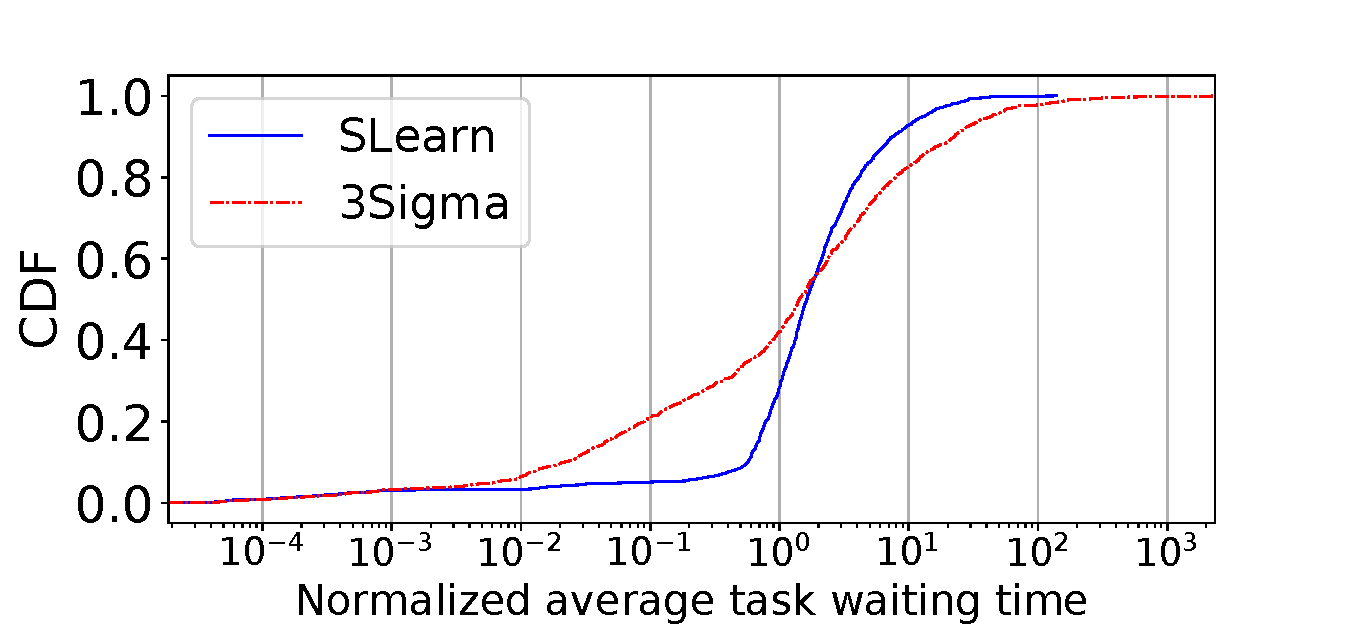
\includegraphics[width=0.31\textwidth]{figures/simulation/normalized_average_task_waiting_time_2STrace.pdf}
	\label{fig:sim:waitingTimes:2STrace:cdf}
	\vspace{-0.1in}
}
	\subfigure[Job A - JCT Speedup - $1.00\times$]{
\vspace{-0.2in}
	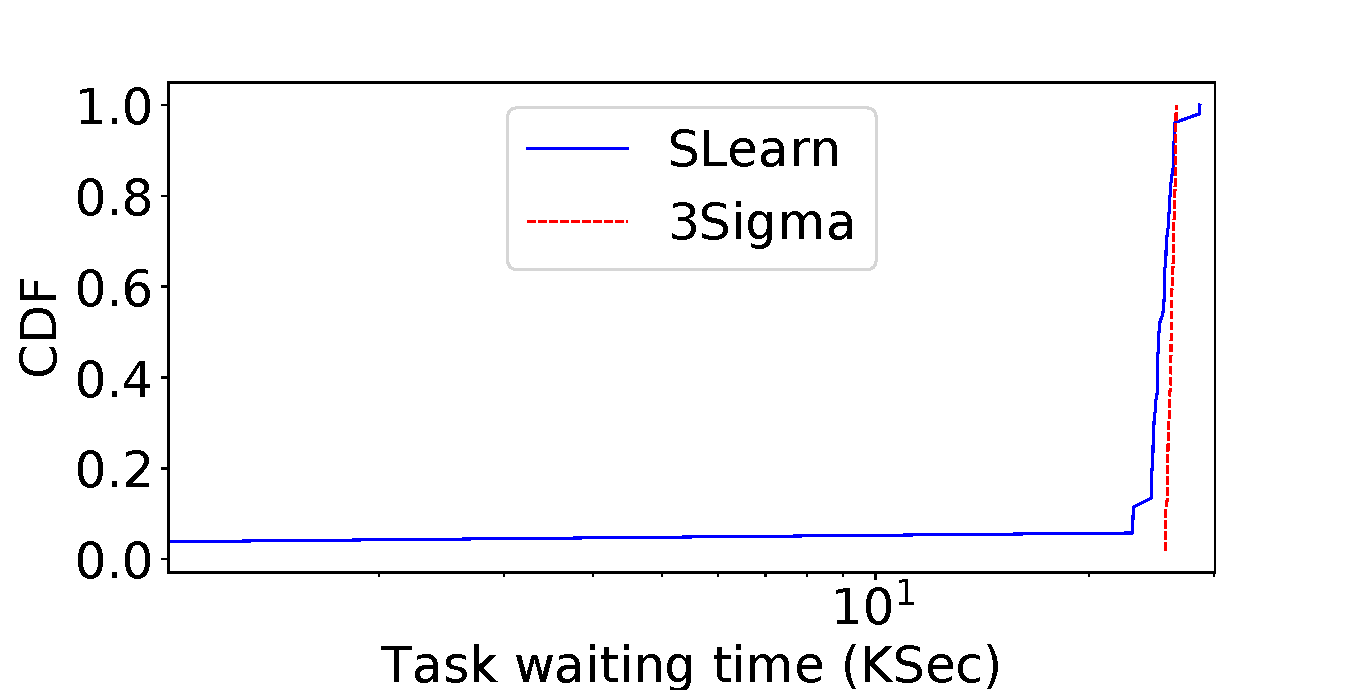
\includegraphics[width=0.31\textwidth]{figures/simulation/task_waiting_time_cdf_JOB-64066.pdf}
	\label{fig:sim:waitingTimes:2STrace:same}
	\vspace{-0.1in}
}
	\subfigure[Job B - JCT Speedup - $6.40\times$]{
	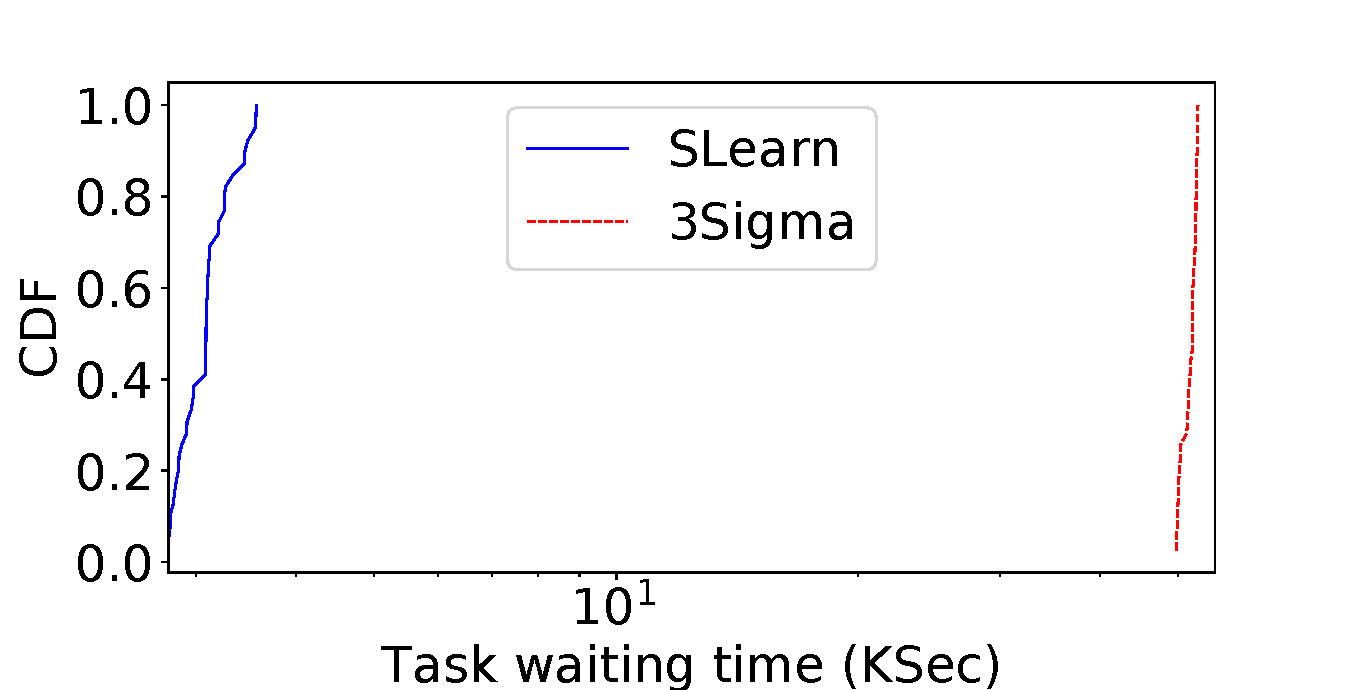
\includegraphics[width=0.31\textwidth]{figures/simulation/task_waiting_time_cdf_JOB-61599.pdf}
	\label{fig:sim:waitingTimes:2STrace:improvement}
	\vspace{-0.1in}
}
\vspace{-0.2in}
\caption{Waiting times for jobs in 2STrace. \updated{all - 16th Sep 2020}}
\label{fig:sim:waitingTimes}
\vspace{-0.1in}
\end{figure*}

A key question about sampling-based learning is whether sampling pilot tasks
first will cause the remaining tasks of a job to wait too long, thus affecting
its JCT.  To answer this question, we next measure and compare the {\em
normalized waiting time} of jobs, calculated as the average waiting time for
each of its tasks divided by job total runtime, under different learning
schemes.
%  We compare the job waiting times under \slearn with that under
%  \primarybasepredict.

Figure~\ref{fig:sim:waitingTimes:2STrace:cdf} shows the CDF of normalized
waiting times for \slearn and \primarybasepredict for  2STrace.  Despite the
sampling overhead, \slearn has considerably lower job waiting time.  In
particular, 40.95\% of all jobs (43.56\% of all the wide jobs) incurred
lower average task waiting time when scheduled under \slearn than under
\primarybasepredict.  The lower waiting time comes from higher estimation
accuracy of \slearn: jobs are scheduled in a better order, and they finish
faster and incur less delay on other jobs. \questionaj{Will it be better to show max waiting time instead of average?}
%  (2) In a busy cluster, not all the jobs are scheduled
%  immediately upon their arrival and they wait anyway. By sampling a small
%  fraction of tasks, the waiting times of other jobs are not elongated much.

Fig.~\ref{fig:sim:waitingTimes:2STrace:same} and
Fig.~\ref{fig:sim:waitingTimes:2STrace:improvement} show the task waiting
dynamics for a job that had similar JCT and a job that experienced a speedup of
5.38$\times$ under \slearn.  We see for both jobs, both the sampled tasks and
most of the non-sampled tasks in \slearn started much earlier as compared to
their starting moments under \primarybasepredict.  The same observation is true
for most of the jobs, which suggests sampling does not inflate the waiting time
of the jobs.

{The results for GTrace are similar to for 2STrace. 57\% of all the jobs and
60\% of wide jobs for GTrace incurred lower waiting time when scheduled under
SLearn than under 3Sigma. We omit the details due to page limit.
%These values are similar to those for 2STrace: 68\% of all the jobs and 72\%
%of the wide jobs.
}
\subsubsection{Sampling Accuracy}
\label{sec:sim:accuracy}

\slearn achieves significantly more accurate estimation of job runtime over 
\primarybasepredict\ --
the details were already discussed in \S\ref{sec:accuracy:experiment}.

\begin{figure*}
%\begin{minipage}{0.72\textwidth}
\vspace{-0.15in}
\centering
\subfigure[\vspace{-0.2in} 2STrace]
{
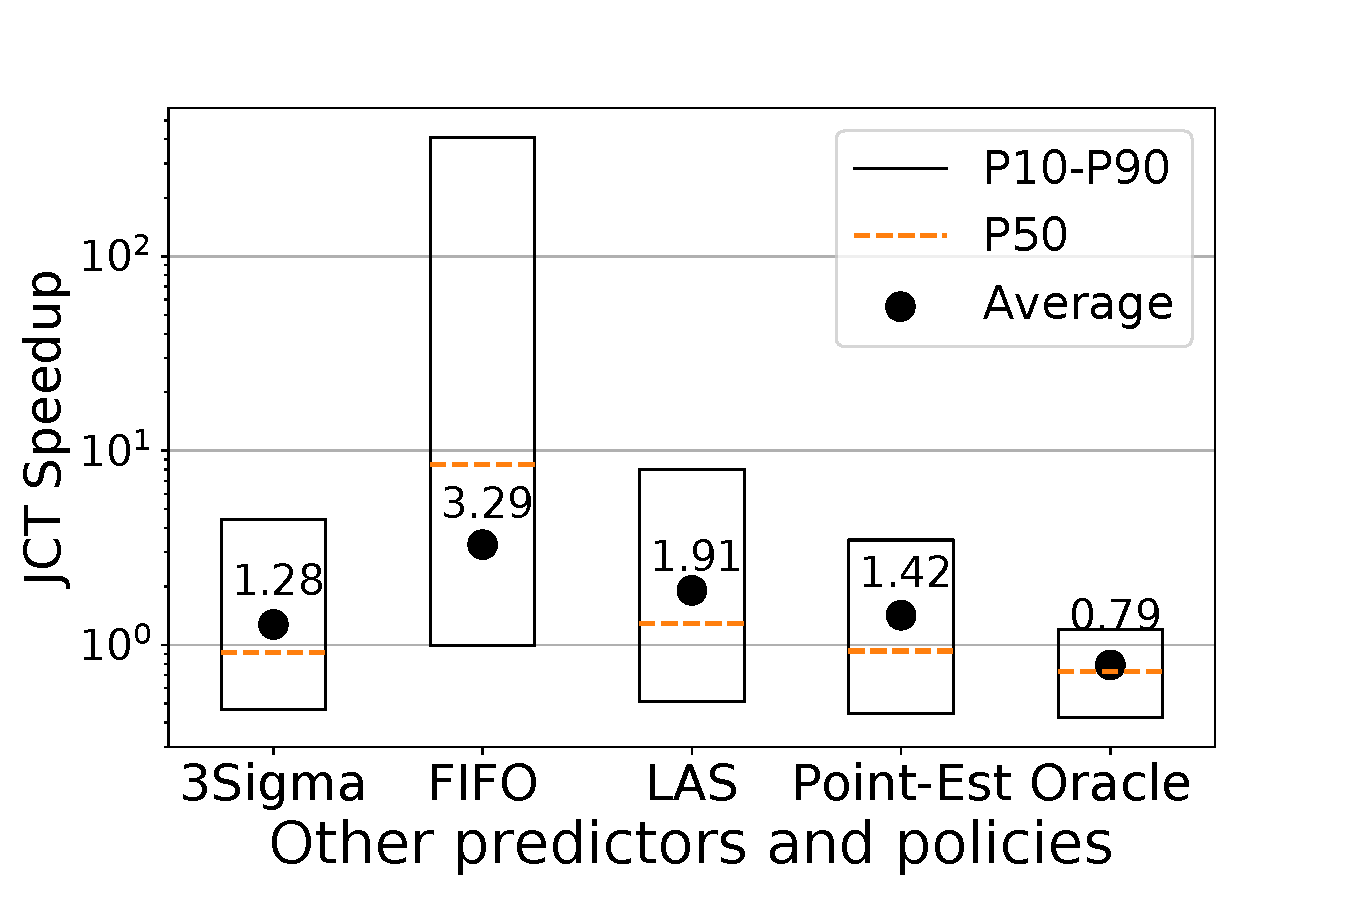
\includegraphics[width=0.32\linewidth]{figures/simulation/PerformanceCompare2SigmaTrace.pdf}
\hspace{-0.1in}
\label{fig:sim:jctOthers:2STrace}
}
\subfigure[\vspace{-0.2in} GTrace11]
{
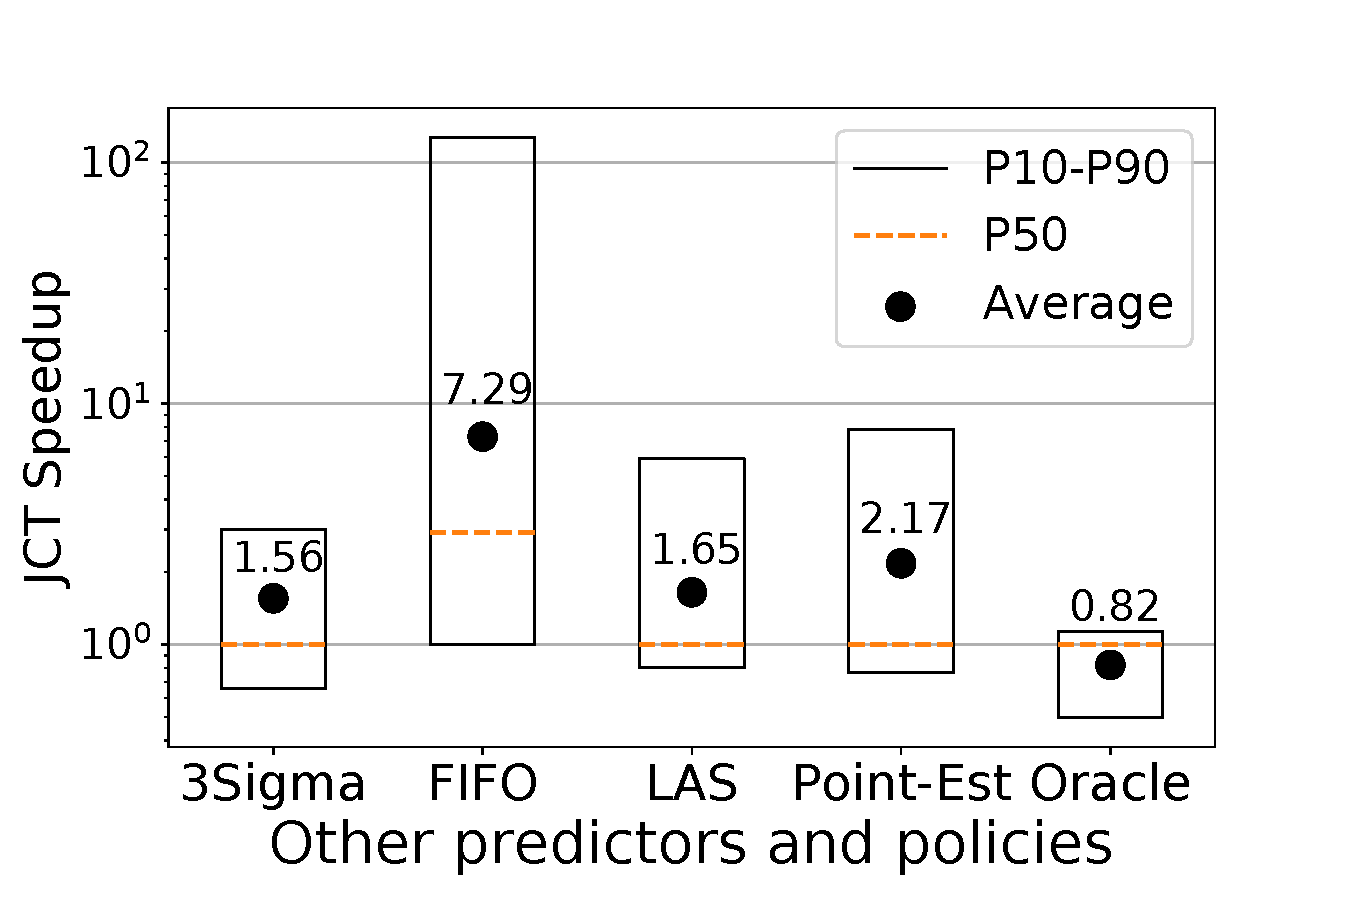
\includegraphics[width=0.32\linewidth]{figures/simulation/PerformanceCompareGTraceVersion2.pdf}
\hspace{-0.1in}
\label{fig:sim:jctOthers:GTrace11}
}
\subfigure[\vspace{-0.2in} GTrace19]
{
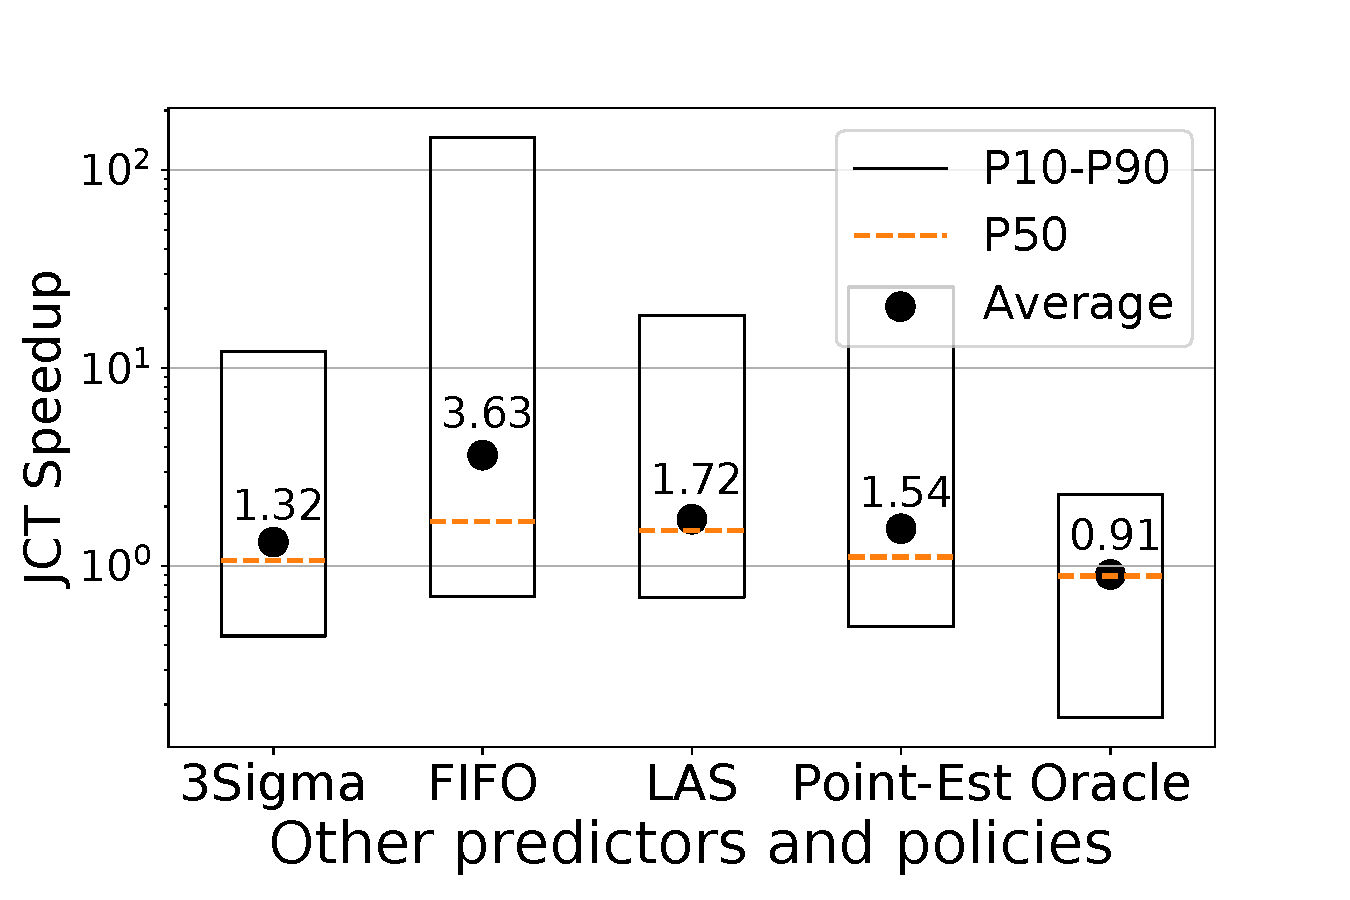
\includegraphics[width=0.32\linewidth]{figures/simulation/PerformanceCompareGTrace2019.pdf}
\hspace{-0.1in}
\label{fig:sim:jctOthers:GTrace19}
}
\vspace{-0.2in}
\caption{JCT speedup using \slearn as compared to other baseline schemes for
	the two traces. \updated{all - 16th Sep 2020}
}
\vspace{-0.1in}
\label{fig:sim:jctOthers}
\end{figure*}
%\end{minipage}
\hfill
\begin{figure}
%\begin{minipage}{0.23\textwidth}
%\centering
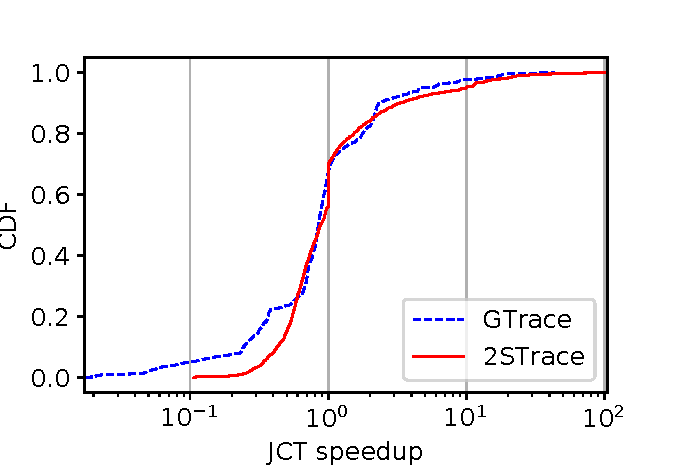
\includegraphics[width=0.9\linewidth]{figures/testbed/testbedBothTracesSpeedupCDF-speedUp-CDF.pdf}
	\captionof{figure}{[Testbed] CDF of speedup of \slearn over \primarybasepredict for 2STrace and GTrace. \updated{13th Jul 2020}}
\label{fig:testbed:speedup:cdf}
%\end{minipage}
\end{figure}
%\end{figure*}

\subsubsection{Average JCT Improvement}
\label{sec:sim:averageJCT}

We now compare the JCT speedups achieved using \slearn over using the
five baseline schemes defined in \S\ref{sec:design:baselines}.
% (1) \primarybase, (2) \pointestimator, (3) \oracle, (4) \las, and (5) \fifo.
%  All experiments use the default parameters discussed in the setup, including
%  $K, E, S$, unless otherwise stated.

\begin{table}[tp]
	\caption{Percentage of the wide jobs that had correct queue assignment \updated{all - 16th Sep 2020 TableStructure - 10 Jul 2020}}
\vspace{-0.1in}
\label{table:sim:correctQueue}
  \centering
      {\small
	\begin{tabular}{|c|c|c|c|c|c|} 
	  \hline
		Prediction&	\slearn &\primarybasepredict &\oracle\\  
		%Prediction&	\slearn &\primarybasepredict &\pointestimator\\  
		Technique&&&\\
	  \hline
		2STrace &89.09\%&73.84\%&100\%\\
		GTrace11 &86.45\%&76.20\%&100\%\\
		GTrace19 &73.96\%&58.07\%&100\%\\
		%Queue Assign-&89.38\%&68.39 (73.85)\%&61.02 (62.8)\%\\
		%ment Accuracy&&&\\
	  \hline
	\end{tabular}
      }
\vspace{-0.1in}
\end{table}
Fig.~\ref{fig:sim:jctOthers:2STrace}
shows the results for 2STrace. We make the following observations.
(1) \oracle predicts with 100\% accuracy and thus all the jobs are placed in
their correct queues.  Therefore, the JCT of \oracle serves as a lower-bound
for all other schemes.
%
Compared to \oracle, \slearn achieves an average JCT speedup and P50 speedup of
0.79$\times$ and 0.73$\times$, respectively.
%  In other words, the JCT of \slearn is not increased significantly even
%  though
This is because \slearn has some estimation error; it places 10.91\% of wide
jobs in the wrong queues. 3.54\% in lower queue and 7.37\% higher queues.
(2) \slearn improves the average JCT over \primarybase by 1.28$\times$ and the
P50 speedup is 0.92$\times$.  This significant improvement of \slearn comes
from much higher prediction accuracy compared to \primarybasepredict
(Fig.~\ref{fig:sim:estimationAccuracy}).
(3) Compared to \pointestimator, \rm{which uses a point estimate generated from
historical data,} \slearn improves the average JCT by 1.42$\times$ and the P50
speedup is 0.93$\times$.
%
Again, this is because \slearn estimates runtimes with higher accuracy. 
%   \slearn achieves higher
%   improvement over \pointestimator than over \primarybase because
%   \primarybase, which exploits complete runtime distribution, can predict with
%   better accuracy than \pointestimator.
%
To illustrate \slearn's high prediction accuracy,
we show in Table~\ref{table:sim:correctQueue} the fraction of wide jobs that were
placed in correct queues by \slearn, \primarybasepredict and \pointestimator.
We observe that \slearn assigns 89.38\% of the wide jobs to correct queues but
\primarybasepredict and \pointestimator assign only 68.39\% and 67.14\% jobs correctly,
respectively.
%
(4) Compared to \las, \slearn achieves an average JCT speedup of
1.91$\times$ and the P50 speedup of 1.29$\times$. This is because \las
pays a heavy penalty in identifying the correct queues of jobs
by moving them across the queues incrementally. In that process, many
large jobs are scheduled before small jobs which results in
needless delay for small jobs.
(5) Lastly, compared with \fifo, where all the jobs are scheduled in the order of
arrival, \slearn achieves an average JCT speedup of 3.29$\times$ and P50
speedup of 8.45$\times$.

\if 0
A recent trace analysis paper~\cite{workloadDiversity:atc18} showed
the distribution of job runtimes can vary from one cluster to another.
To evaluate \slearn's robustness to trace distribution, we compared
\slearn against all four baseline schemes using GTrace.  
\fi

Fig.~\ref{fig:sim:jctOthers:GTrace11} shows the results for GTrace11.  
% We see that 
Scheduling under \slearn again outperforms all other schemes. In particular,
using \slearn improves the average JCT by 1.56$\times$ compared to using
\primarybasepredict, 2.17$\times$ compared to using the Point-Estimate
predictor, and 1.65$\times$ compared to using the LAS policy.
Scheduling under \slearn outperforms all other schemes for GTrace19 too
(Fig.~\ref{fig:sim:jctOthers:GTrace19}). In particular, using \slearn improves
the average JCT by 1.56$\times$ compared to using \primarybasepredict,
2.17$\times$ compared to using the Point-Estimate predictor, and 1.65$\times$
compared to using the LAS policy.

In summary, our results above show that \slearn's higher estimation accuracy
outweighs its runtime overhead from sampling, and as a result achieves much
lower job completion time than history-based predictors and the LAS policy for
the two production workloads.

\commentaj{Cluster G from 2019 has very high error. However, that is not the
case with all the cluster of 2019. I tried with other clusterH with all tier
jobs. That also has a speed up 1.25$\times$ and P50 (P90) error for \slearn is
1.23 (9.39)\% and for \primarybasepredict it is 8.63 (53.60)\%. With clusterB
beb-tier jobs the speedup is 1.9$\times$ and P50 (P90) error for \slearn is
7.65 (58.68)\% and for \primarybasepredict it is 28.72 (144.01)\%. I think we
can use this result somewhere as clusterG 2019 has very high error for both
\slearn and \primarybasepredict.}

\subsubsection{Intuitive explanation of speedup}
\label{sec:sim:intuitionSpeedup}

\begin{figure*}
	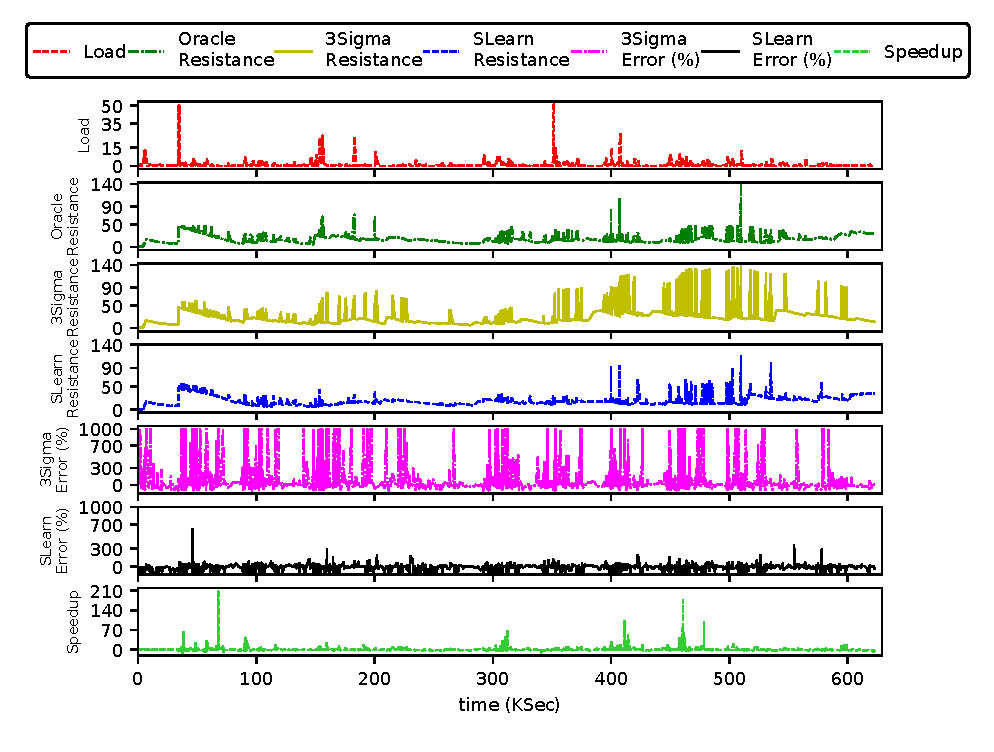
\includegraphics[width=1.0\linewidth]{figures/simulation/2STrace-Trial.eps}
	\caption{Correlation between load, \textit{resistance}, estimation error and speedup for 2STrace. \updated{16th Sep 2020}}
	\label{figs:sim:intuitionSpeedup:allInOne}
\end{figure*}

\S\ref{sec:sim:numPilots} - \S\ref{sec:sim:averageJCT} explain better performance under 
\slearn over \primarybase by experimental results. In this section, we provide
an intuitive explanation of the improvement.
Figure~\ref{figs:sim:intuitionSpeedup:allInOne} shows seven timeline values comparing
\slearn and \primarybase as follows:

\begin{itemize}
	\item The top curve shows the total workload arrived in the past 1000
		seconds, in terms of execution duration, for the 2STrace. The
		values are plotted in steps of 1000 seconds along the x-axis.
		A unit along the y-axis is corresponding to the workload which
		needs 1000 seconds of the entire cluster's compute capacity.
	\item The next three curves show the \resistance faced by jobs under
		\oracle, \primarybase and \slearn, respectively.  Where
		\resistance for a job is defined as the amount of higher
		priority workload existing at the time of its arrival
		\comment{including} the sum of the remaining duration of the
		already scheduled tasks. A unit along the y-axis for these
		curves is also corresponding to the workload which needs 1000
		seconds of the entire cluster's compute capacity. For wide
		jobs, under \slearn we show the value corresponding to the time
		when the job's size estimation is over and it has been placed
		in its estimated priority queue. The values are plotted along
		the x-axis corresponding to each job's arrival time.
	\item The next two curves correspond to the percentage error in
		\primarybasepredict and \slearn respectively.  They show signed
		error which are capped at 1000, \eg a value of -20 on error
		curves means the job was estimated to be 20\% smaller and a
		value of 1000 means job was estimated at least 10 $\times$
		larger. The values are plotted along the x-axis corresponding
		to each job's arrival time.
	\item The bottom curve shows the job speedup of \slearn over
		\primarybase.  Negative values mean the job slowed down under
		\slearn compared to \primarybase. The values are plotted along
		the x-axis corresponding to each job's arrival time.\\
%	\questionaj{Should we also add speedup of \slearn vs. \oracle and
		%	\primarybase vs. \oracle. If yes, should we then move
		%	the \primarybase vs. \slearn speedup curve.}
\end{itemize}

With the above definitions of the curves, we next discuss what these curves
demonstrate intuitively.  The values on the \resistance curve indicate the
amount of workload which will be scheduled before the arriving job gets to run.
So, a job's completion time is roughly proportional to the \resistance it sees
upon arrival.  The \resistance, in turn, depends on the recently arrived
workload and the prediction error. It is obvious that if more workload has
arrived in the recent past, before a job's arrival, it is highly likely that
the job will face higher \resistance.  More importantly, when the job is
estimated larger than its usual size, it may be misplaced in a lower priority
queue. If the error is more than 1000\% then the job will definitely be placed
in a lower priority queue. In such cases, the job will likely face higher
\resistance than it would have with accurate estimation.  Also, the jobs which
are underestimated may get placed in a higher priority queue. Though these jobs
will finish faster themselves but will create more \resistance for many other
jobs which are smaller than it and will slow them down. Only this part is hard
to visualize from the curves, but the other intuitions are easy to visualize
from the plots in figure \ref{figs:sim:intuitionSpeedup:allInOne}.  We can see
that the \resistance under \slearn is very similar to \oracle however under
\primarybase it is not.  Also, it is clearly visible that the peaks on
\resistance curve for \primarybase are mostly at the points where there is high
positive prediction error under \primarybase too.  Next, we can also see that
where there is higher \resistance  under \primarybase as compared to the
\slearn, those are the points where most of the peaks in the curve showing
speedup of \slearn over \primarybase are also observed.

%The data shown in table \ref{table:sim:overestimatedJobs} and
%\ref{table:sim:underestimatedJobs} also establishes the intuitive observations
%made from the curves.  \primarybase overestimates 59.37\% of the total jobs.
%Among the overestimated jobs, 36.02\% are misplaced at a lower priority queue,
%and among the misplaced jobs 82.84\% slowdown when compared to \oracle.
%Whereas \slearn overestimates 43.75\% of the total jobs. Among those only
%8.09\% are misplaced at a lower priority queue and are slowed down as compared
%to \oracle.
%%On the other side \primarybase underestimates 40.63\% of the jobs.
As visible from Fig.~\ref{figs:sim:intuitionSpeedup:allInOne}, most of the jobs
have low prediction error under \slearn whereas a significant number of jobs
have large prediction error under \primarybase. This explains why a larger
number of jobs, as shown in table \ref{table:sim:misplacedJobs:all}
%\ref{table:sim:overestimatedJobs} and \ref{table:sim:underestimatedJobs}, 
get misplaced under \primarybase and eventually deteriorate overall
performance.

%\questionaj{The current values in table \ref{table:sim:overestimatedJobs} and
%\ref{table:sim:underestimatedJobs} for \slearn are only for wide jobs and for
%\primarybase they are for all the jobs. What should we be doing here?}

\begin{table*}
\caption{Fraction of overestimated jobs and incorrect queue placement for 2STrace. Job performance in the third and seventh column is relative to the \oracle. \updated{2S - 16th Sep 2020}}
  \label{table:sim:misplacedJobs:all}
\vspace{-0.1in}	
  \centering
      {\small
	\begin{tabular}{|c|c|c|c|c|c|c|c|c|} 
	  \hline
		& Overestim- & Misplaced over- & Slowed mis- & Average (P50) & Underesti- & Misplaced under & Spedup mis- & Average (P50)\\
		& ated jobs & estimated jobs & placed jobs & Positive error & mated jobs & estimated jobs & placed jobs & Negative error\\
	  \hline
		%\primarybase & 59.37\% & 21.09\% & 17.72\% & 1253.60 (66.38)\% & 40.63\% & 10.22\% & 8.46\% & -39.33 (-31.59)\%\\
		\primarybase & 59.78\% & 17.50\% & 12.19\% & 898.45 (48.00)\% & 40.22\% & 8.65\% & 6.88\% & -37.0 (-28.57)\%\\
	  \hline
	  	\slearn & 43.75\% & 3.54 \% & 2.85\% & 30.65 (18.19)\% & 55.45\% & 7.37\% & 3.64\% & -26.79 (-20.69)\% \\
	  \hline
	\end{tabular}
      }
\vspace{-0.1in}	
\end{table*}

%\questionaj{I can add more numbers in the above line \eg jobs placed in a lower PQ but still performing better. Or jobs place in right queue but performing poor and similar number for jobs which were under estimated. But I think those will make things clumsy, please let me know what do you think?}
%maybe not 

In conclusion, whether a job finishes faster under \slearn compared to
\primarybase is a function of the prediction error. Due to high prediction
error in \primarybase, jobs get ordered incorrectly and hence face higher
\resistance, which results in longer finishing time under \primarybase.

%By looking at the 3Sigma resistance and error it becomes very evident that jobs
%which are estimated atleast 10$\times$ larger face much higher resistance as
%compared to what is observed for them in Oracle. This is because when estimated
%atleast 10$\times$ larger, the job will be moved to atleast 1 hop lower priority
%queue than it's actual queue. Since these queues are FIFO so all the workload of 
%the lower priority queue also adds to the resistance faced by the arriving job.
%In our experiments with the 2STrace \primarybase estimates 8(14)\% wide jobs 10(2-10) 
%$\times$ larger and all(half) of them are placed in a lower priority queue and
%more then 75(65)\% of them are slowed down compared to \slearn.
%
%No jobs in \slearn are estimated 10$\times$ or more larger.

\subsubsection{Testbed Experiments}
\commentaj{This section is not updated.\\}
We next performed end-to-end evaluation of \slearn and 3Sigma on our 150-node
Azure cluster.  Fig.~\ref{fig:testbed:speedup:cdf} shows the CDF of JCT
speedups using \slearn over \primarybasepredict using 2STrace and GTrace.
\slearn's performance on the testbed is similar to what is observed in
simulation.  In particular, \slearn achieved {average} JCT speedups of
1.40$\times$ and 1.26$\times$ over \primarybase for 2STrace and GTrace,
respectively.

\subsubsection{Binning Analysis}
\label{sec:sim:binning}

To gain insight into how different jobs are affected by \slearn over
\primarybase, we group the jobs into four bins defined in
Table~\ref{table:sim:bin:2STrace}, \ref{table:sim:bin:GTrace11}, \ref{table:sim:bin:GTrace19}, and study the JCT speedups for each bin.

\begin{table}
	\caption{Breakdown of jobs based on total duration and width (number of tasks) for 2STrace \updated{16th Sep 2020}}
% The 	numbers in brackets denote the fraction of jobs in that bin for the 2STrace. \updated{10th May 2019 for 2STrace and on 13th for GTrace}}
  \label{table:sim:bin:2STrace}
\vspace{-0.1in}	
  \centering
      {\small
	\begin{tabular}{|c|c|c|c|c|} 
	  \hline

		& width $<$ \thinLimit (thin) & width $\geq$ \thinLimit (wide) \\
	  \hline
		size $> 10^6 ms $ (small) & bin-1 (4.55\%) & bin-2 (28.73\%) \\
	  \hline
	  	size $\leq 10^6 ms $ (large) & bin-3 (14.29\%) & bin-4 (52.43\%) \\
	  \hline
	\end{tabular}
      }
\vspace{-0.1in}	
\end{table}

\begin{table}
	\caption{Breakdown of jobs based on total duration and width (number of tasks) for GTrace11 \updated{16th Sep 2020} \commentaj{This distribution is very distorted because we have dropped jobs with single task}}
  \label{table:sim:bin:GTrace11}
\vspace{-0.1in}	
  \centering
      {\small
	\begin{tabular}{|c|c|c|c|c|} 
	  \hline

		& width $<$ \thinLimit (thin) & width $\geq$ \thinLimit (wide) \\
	  \hline
		size $> 10^6 ms $ (small) & bin-1 (35.25\%) & bin-2 (8.00\%) \\
	  \hline
	  	size $\leq 10^6 ms $ (large) & bin-3 (1.60\%) & bin-4 (55.15\%) \\
	  \hline
	\end{tabular}
      }
\vspace{-0.1in}	
\end{table}

\begin{table}
	\caption{Breakdown of jobs based on total duration and width (number of tasks) for GTrace19 \updated{16th Sep 2020} \commentaj{This distribution is very distorted because we have dropped jobs with single task}}
  \label{table:sim:bin:GTrace19}
\vspace{-0.1in}	
  \centering
      {\small
	\begin{tabular}{|c|c|c|c|c|} 
	  \hline

		& width $<$ \thinLimit (thin) & width $\geq$ \thinLimit (wide) \\
	  \hline
		size $> 10^6 ms $ (small) & bin-1 (0.80\%) & bin-2 (3.74\%) \\
	  \hline
	  	size $\leq 10^6 ms $ (large) & bin-3 (1.99\%) & bin-4 (93.47\%) \\
	  \hline
	\end{tabular}
      }
\vspace{-0.1in}	
\end{table}

\begin{figure*}[tp]
\vspace{-0.1in}
\subfigure[2STrace]
{
	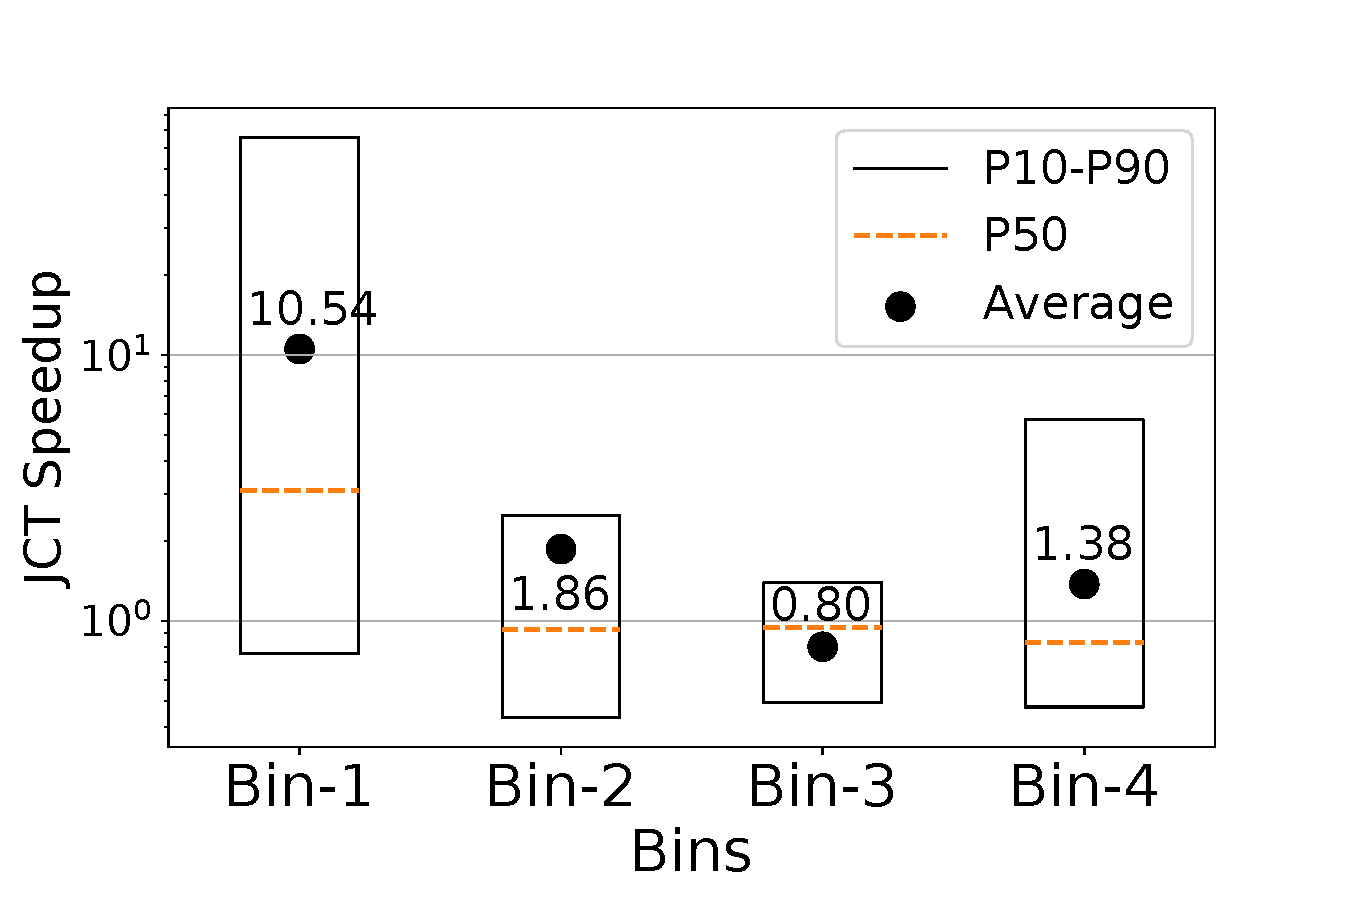
\includegraphics[width=0.33\linewidth]{figures/simulation/binning2SigmaTrace.pdf}
	\label{figs:sim:bin:2STrace}
}
\hspace{-0.25in}
	\subfigure[GTrace11]
{
	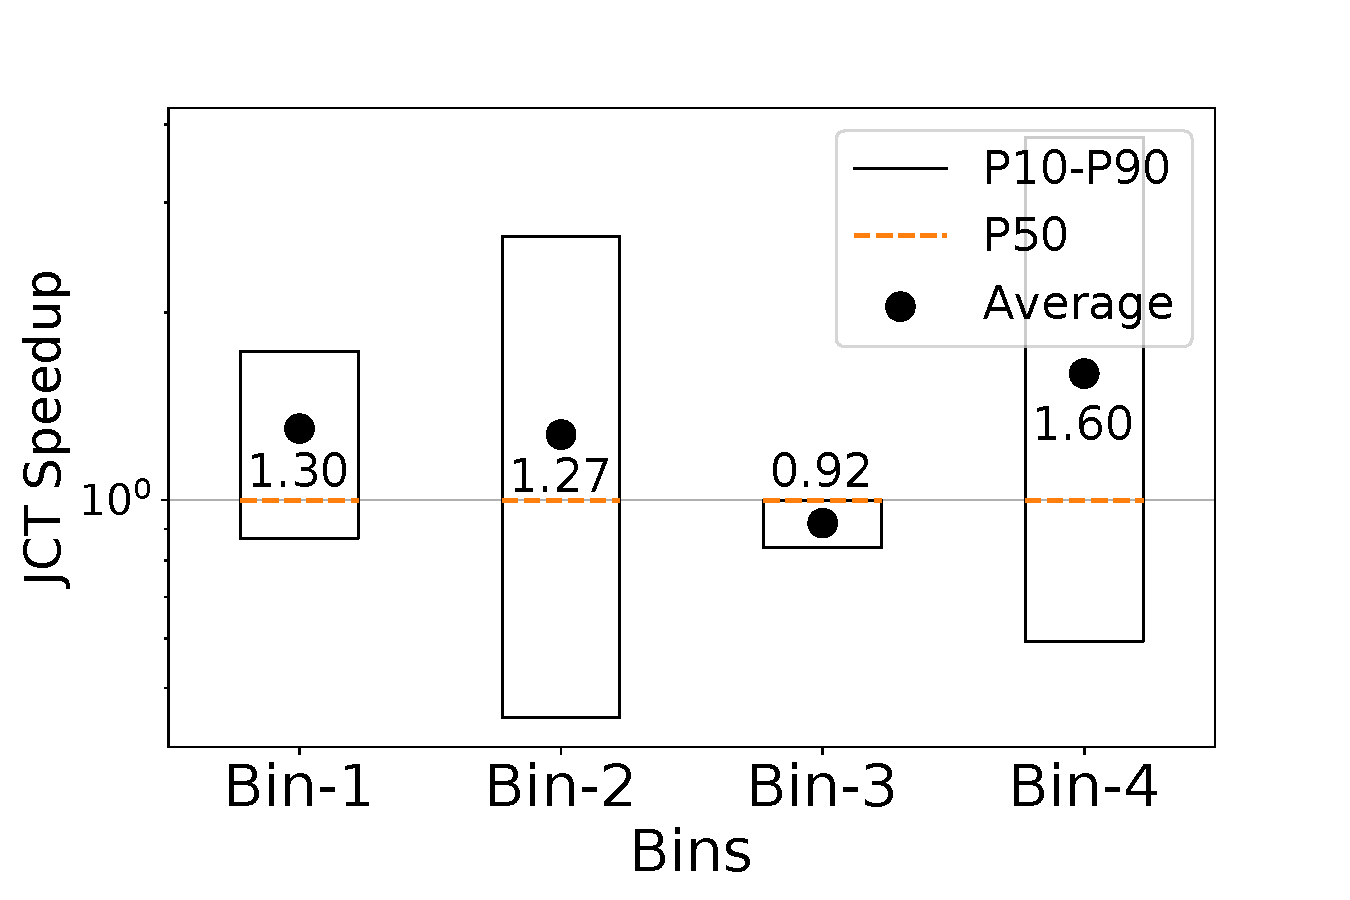
\includegraphics[width=0.33\linewidth]{figures/simulation/binningGTraceVersion2.pdf}
	\label{figs:sim:bin:GTrace11}
}
\hspace{-0.25in}
	\subfigure[GTrace19]
{
	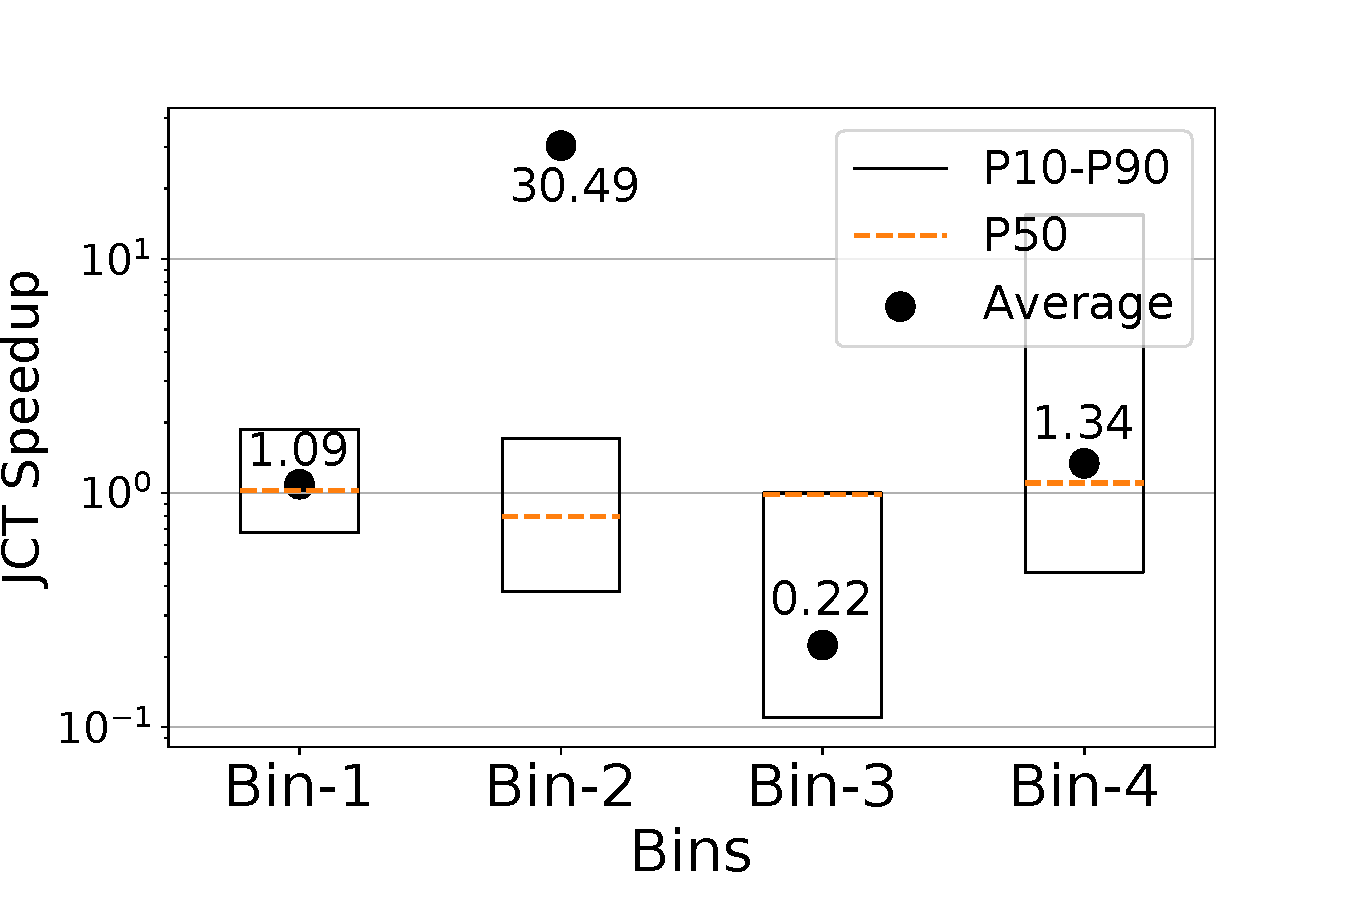
\includegraphics[width=0.33\linewidth]{figures/simulation/binningGTrace2019.pdf}
	\label{figs:sim:bin:GTrace19}
}
\vspace{-0.15in}
\caption{Performance breakdown into bins in Table~\ref{table:sim:bin:2STrace}, \ref{table:sim:bin:GTrace11} and \ref{table:sim:bin:GTrace19} respectively.\updated{16th Sep 2020}}
\vspace{-0.20in}
\label{figs:sim:bin}
\end{figure*}


Fig.~\ref{figs:sim:bin:2STrace} shows the results for 2STrace.  \slearn improves JCT
for 82.46\% in Bin-1, 45.56\% in Bin-2 and 29.05\% Bin-3,
and 41.10\%  of the jobs in Bin-4.
We make the following observations.
(1) Bin-3 (thin-large), which has 14.28\% of the jobs and accounts for 5.41\% of the total
job size, has a slowdown of 20.00\%. This is the reason that even though Bin-4,
which has 52.43\% of the jobs and accounts for 94.52\% of the total job size,
has speedup of 1.38$\times$. The overall speedup is 1.28$\times$.  Bin-1 and
Bin-2 have very insignificant fraction in total jobs size hence their high
speedups don't make much difference. The primary reason for slowdown of
\slearn in Bin-3 is that \slearn treats thin jobs in FIFO order, whereas,
\primarybase schedules them based on predicted size. Additionally, \primarybase
misplaces 80.35\% of the largest 62.57\% jobs of Bin-3 in higher priority
queues, which results in speeding up these jobs under \primarybase. 

%(2) The reason that all the jobs in Bin-3 have speedups under \slearn compared to
%\primarybase is that these jobs are thin and large. Since they are thin,
%\slearn gives them high priority. In contrast, provided they are large, \primarybase
%schedules them at lower priority.
(2) Bin-2 (wide-small) jobs are almost equally affected by improved accuracy of \slearn.
%(3) The mixed results for Bin-1 is because \slearn puts all the thin jobs in the
%highest priority queue. However, some can slow down due to being blocked by
%other thin but large jobs. The jobs with speedups are those either rightly
%prioritized as being small {by \slearn} or mis-identified as low priority by
%\primarybase. We note that though \slearn bypasses all the thin jobs, they
%only account for less than 2\% of the total job size.

% {We omit detailed results of this analysis for GTrace due to
% space limitation. Results are summarized at the end of the subsection.}

Fig.~\ref{figs:sim:bin:GTrace11} shows the results for GTrace11.
% Since GTrace has a higher fraction of thin jobs as compared to 2STrace, the
% bin distribution of jobs is a little different.  However, 
Here Bin-4 dominates the overall average JCT improvement as it accounts for
55.15\% of the jobs and 98.57\% of the total job size.  Its average JCT
improvement of 1.60 $\times$ directly contributes to the total average JCT
improvement of 1.60$\times$. Similar is the case with GTrace19
(Fig.~\ref{figs:sim:bin:GTrace19}).

Additionally, a glance at the tables \ref{table:sim:bin:2STrace},
\ref{table:sim:bin:GTrace11}, and \ref{table:sim:bin:GTrace19} can show that the
three traces have very different distribution across the bins. Still, \slearn
has outperformed all the baselines (\S\ref{sec:sim:averageJCT}) for all the
three traces. 

%  for default thinLimit of 6 and 1.53X for thinLimit 3,

\subsubsection{Effect of Thin Job Bypass}
\label{sec:sim:thin}

Finally,
%   we evaluate the effect of \slearn's policy to bypass thin jobs from
%   sampling and schedule them with the highest priority. We conducted two
%   experiments: (1) evaluating \slearn against all the baselines on
%   a ``Wide-Only'' 2STrace, (2) evaluating \slearn's sensitivity to thinLimit.
we evaluate \slearn's sensitivity to thinLimt by varying thinLimit. The results
in Table~\ref{table:sim:sa:tl} shows that for GTrace11 and GTrace19 the average
JCT speedup doesn't vary heavily with thinLimit. For the 2STrace also fluction
is not high when the limit is decrease by 1. However, there is a big dip at
thinLimit four and five.  This is because a significant number of jobs in our
execution trace have width four. Impact of thinLimit variation is different on
the 2 traces because they have different runtime distribution for the thin
jobs. When the thinLimit is 3, thin jobs make 5.41\% of the total runtime for
the 2STrace, 1.17\% for the GTrace11 and 0.56\% for the GTrace19. However, when
thinLimit is 6, the share of thin jobs in total runtime increases only a
little, to 2.69\%, for the GTrace11 and 1.03\% for the GTrace19 whereas
significantly increases, to 13.84\%, for the 2STrace.


\if 0
\subsubsection{Sampling Overhead - Resource Usage}
\label{sec:sim:resource}

\slearn schedules 5\% tasks of each job at the highest priority upon their
arrival. To isolate the effects of this special treatment of sampling tasks and
dedicated usage of resources for sampling. We conducted following experiments.
%Regarding showing that how is 5\% resource used for sampling affecting or not. I did two experiments.
We used a sampling oracle, which has exactly same setting same as \slearn and has
only one difference. In the sampling oracle, sampling tasks are assigned and
the job runtime is estimated by taking mean of durations of the sampling tasks.
But the tasks are not actually executed at the highest priority rather they are
executed during normal execution of the job according to its estimated priority.

Here the average JCT speedup over 3Sigma is 1.98$\times$. The additional gain
over normal execution is due to scheduling of the sampling tasks in the correct
order.

(2) I run our design with 5\% less resources. Improvement over 3 Sigma in this case is 1.54x


the Default improvement is 1.66x

Using these two new results we can explain. I will discuss this in details morning.

\fi

\begin{table}
	\caption{Sensitivity analysis for thinLimit. Table shows average JCT speedup over \primarybase. \updated{all - 16th Sep 2020}}
\vspace{-0.1in}	
	\label{table:sim:sa:tl}
  \centering
      {\small
	\begin{tabular}{|c|c|c|c|c|c|} 
	  \hline
		thinLimit&	2 & 3 & 4 & 5 & 6\\
	  \hline
	  2STrace&	1.23x&1.28x&1.14x&0.97x&0.84x\\%1.45
	  \hline
	  %	2STrace P(50)&	1.40x&1.41x&1.44x&1.40x&1.35x\\
          %GTrace&	1.53x&1.49x&1.40x&1.40x&1.41x\\
          GTrace&	1.54x&1.56x&1.55x&1.54x&1.53x\\
	  \hline
          GTrace19&	1.33x&1.32x&1.32x&1.30x&1.29x\\
	  \hline
	\end{tabular}
      }
\vspace{-0.1in}
\end{table}


\if 0
\begin{table}
  \caption{Sensitivity analysis for thinLimit on GTrace. Table shows average JCT speedup over \primarybase. \updated{2S - 12th May 2020}.
    }
\label{table:sim:sa:tl:GTrace}
  \centering
      {\small
	\begin{tabular}{|c|c|c|c|c|c|} 
	  \hline
          thinLimit &		2 & 3 & 4 & 5 & 6 \\
	  \hline
          Avg. JCT speedup	&	1.31x&1.43x&1.42x&1.42x&1.40x\\
%	  \hline
	  %	P(50)&	0.44x&0.93x&0.94x&0.94x&0.74x\\
	  \hline
	\end{tabular}
      }
\end{table}
\fi
\if 0
\begin{table}
  \caption{Sensitivity analysis for thin node percentage on the GTrace.
    }
  \label{table:sim:sa:tnp}
  \centering
      {\small
	\begin{tabular}{|c|c|c|c|c|} 
	  \hline
thinLimit &		10 & 20 & 30 & 40 & 50\\
	  \hline
Avg. JCT speedup	 	0.72x&1.20x&1.49x&1.66x&1.65x\\
	  \hline
	\end{tabular}
      }
\end{table}
\fi

\vspace{-0.05in}
\if 0
\paragraph{Sampling node percentage} We next vary the threshold for the
sampling node percentage from 10 to 50. Table~\ref{table:sim:sa:snp}
show the results.
\fi

\if 0
\paragraph{Sampling percentage} In this experiment, we vary the sampling percentage 
of queues decreases. As shown in Table~\ref{table:sim:sa:sp}. 
\fi

\if 0
\paragraph{Thin job bypassing limit ($T$)}
In this experiment, we vary the thinLimit (T) in \slearn for bypassing jobs from
the probing phase. The results in Fig.~\ref{table:sim:sa:tl} shows that the
average JCT remains almost the same as T increases.  However, the P50 speedup
increases till $T = \thinLimit$, and tapers off after $T = \thinLimit$.
The key reason for the JCT improvement until $T = \thinLimit$ is that
all tasks of the thin job (with width $< \thinLimit$) are scheduled immediately
upon arrival which improves their JCT (\S\ref{sec:design:thin}).
\fi

\if 0
\paragraph{Thin node percentage} We next vary the threshold for
the thin node percentage from 10 to 50. Table.~\ref{table:sim:sa:tnp}
\fi
